\subsection{Sơ đồ hoạt động}
% https://www.uml-diagrams.org/activity-diagrams.html
\begin{figure}[h!]
	\caption{Sơ đồ hoạt động tổng quát}
	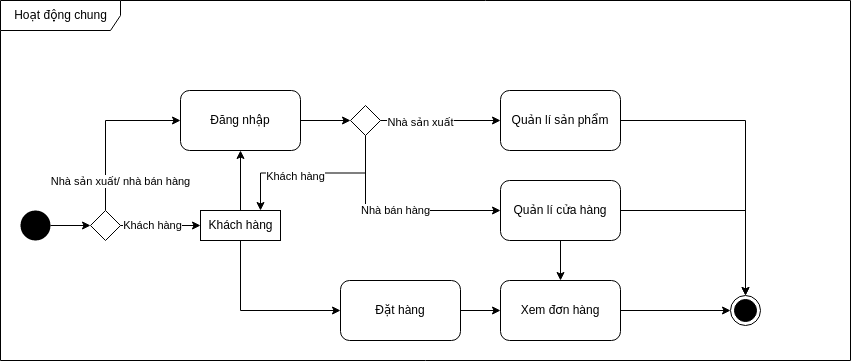
\includegraphics[width=\textwidth]{activity}
\end{figure}

\begin{figure}[h!]
	\begin{center}	
		\caption{Sơ đồ hoạt động người dùng}
		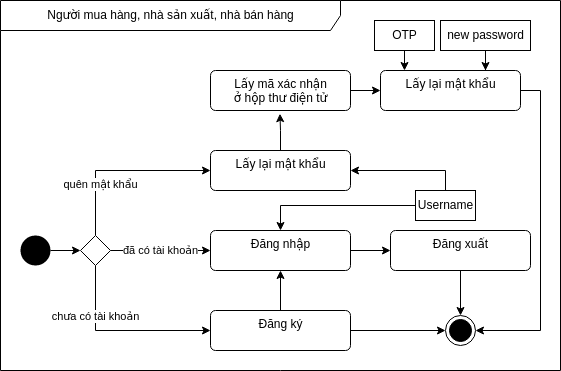
\includegraphics[width=0.8\textwidth]{activity-actors}
	\end{center}
\end{figure}

\begin{figure}[h!]
	\begin{center}	
		\caption{Sơ đồ hoạt động thông báo}
		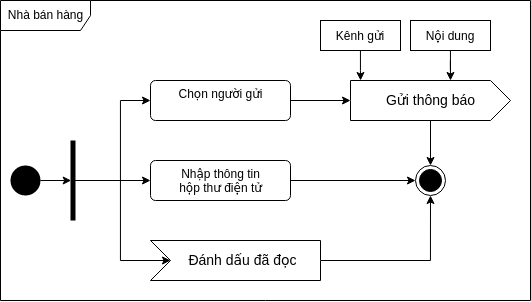
\includegraphics[width=0.8\textwidth]{activity-notification}
	\end{center}
\end{figure}

\begin{figure}[h!]
	\begin{center}	
		\caption{Sơ đồ hoạt động kết bạn}
		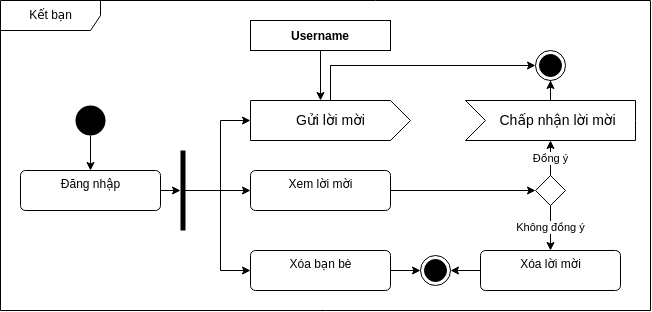
\includegraphics[width=0.8\textwidth]{activity-relationship}
	\end{center}
\end{figure}

\begin{figure}[h!]
	\begin{center}	
		\caption{Sơ đồ hoạt động kí gửi}
		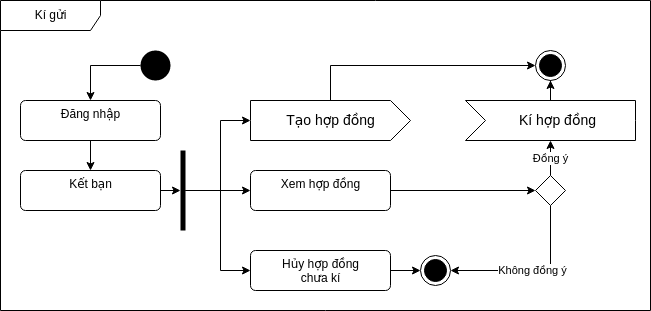
\includegraphics[width=0.8\textwidth]{activity-contract}
	\end{center}
\end{figure}

\begin{figure}[h!]
	\begin{center}	
		\caption{Sơ đồ hoạt động quản lí sản phẩm}
		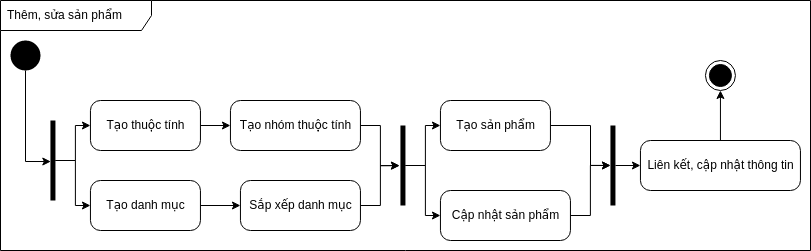
\includegraphics[width=0.6\textwidth]{activity-sellers}
	\end{center}
\end{figure}

\begin{figure}[h!]
	\begin{center}	
		\caption{Sơ đồ hoạt động mua hàng}
		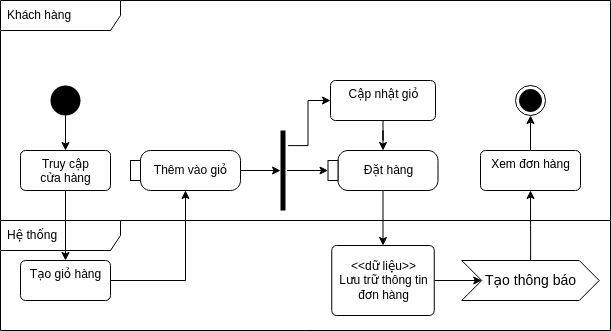
\includegraphics[width=0.6\textwidth]{activity-order}
	\end{center}
\end{figure}

\begin{figure}[h!]
	\begin{center}	
		\caption{Sơ đồ hoạt động quản lí cửa hàng}
		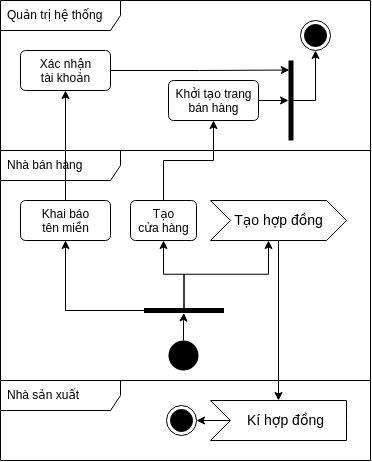
\includegraphics[width=0.6\textwidth]{activity-store}
	\end{center}
\end{figure}